\chapter{脉搏波时域特征集的构建与处理}
\section{引言}
本章将进行PPG波形的新型时域特征的研究,从新型时域特征的设计基础、PPG波形特征描述向量及PPG波形间描述特征等三方面进行说明。
在此基础上,构建基于时长、角度、斜率与面积等维度的PPG多维度时域特征集;
同时将PPG信号的采样序列作为特殊的描述特征,构建PPG采样序列时域特征集,并详细介绍这两类特征集的构建过程。
另外,将被试PPG数据的单个波形与全波波形分别作为子痫前期的最小分析单位,提出基于波形与被试的两个子痫前期识别模型的研究角度,
并按构建机器学习模型的要求,对上述两个特征集进行预处理。

本章研究内容的框架如\autoref{fig:frameworks4}所示。

\begin{figure}[htbp]
  \centering
  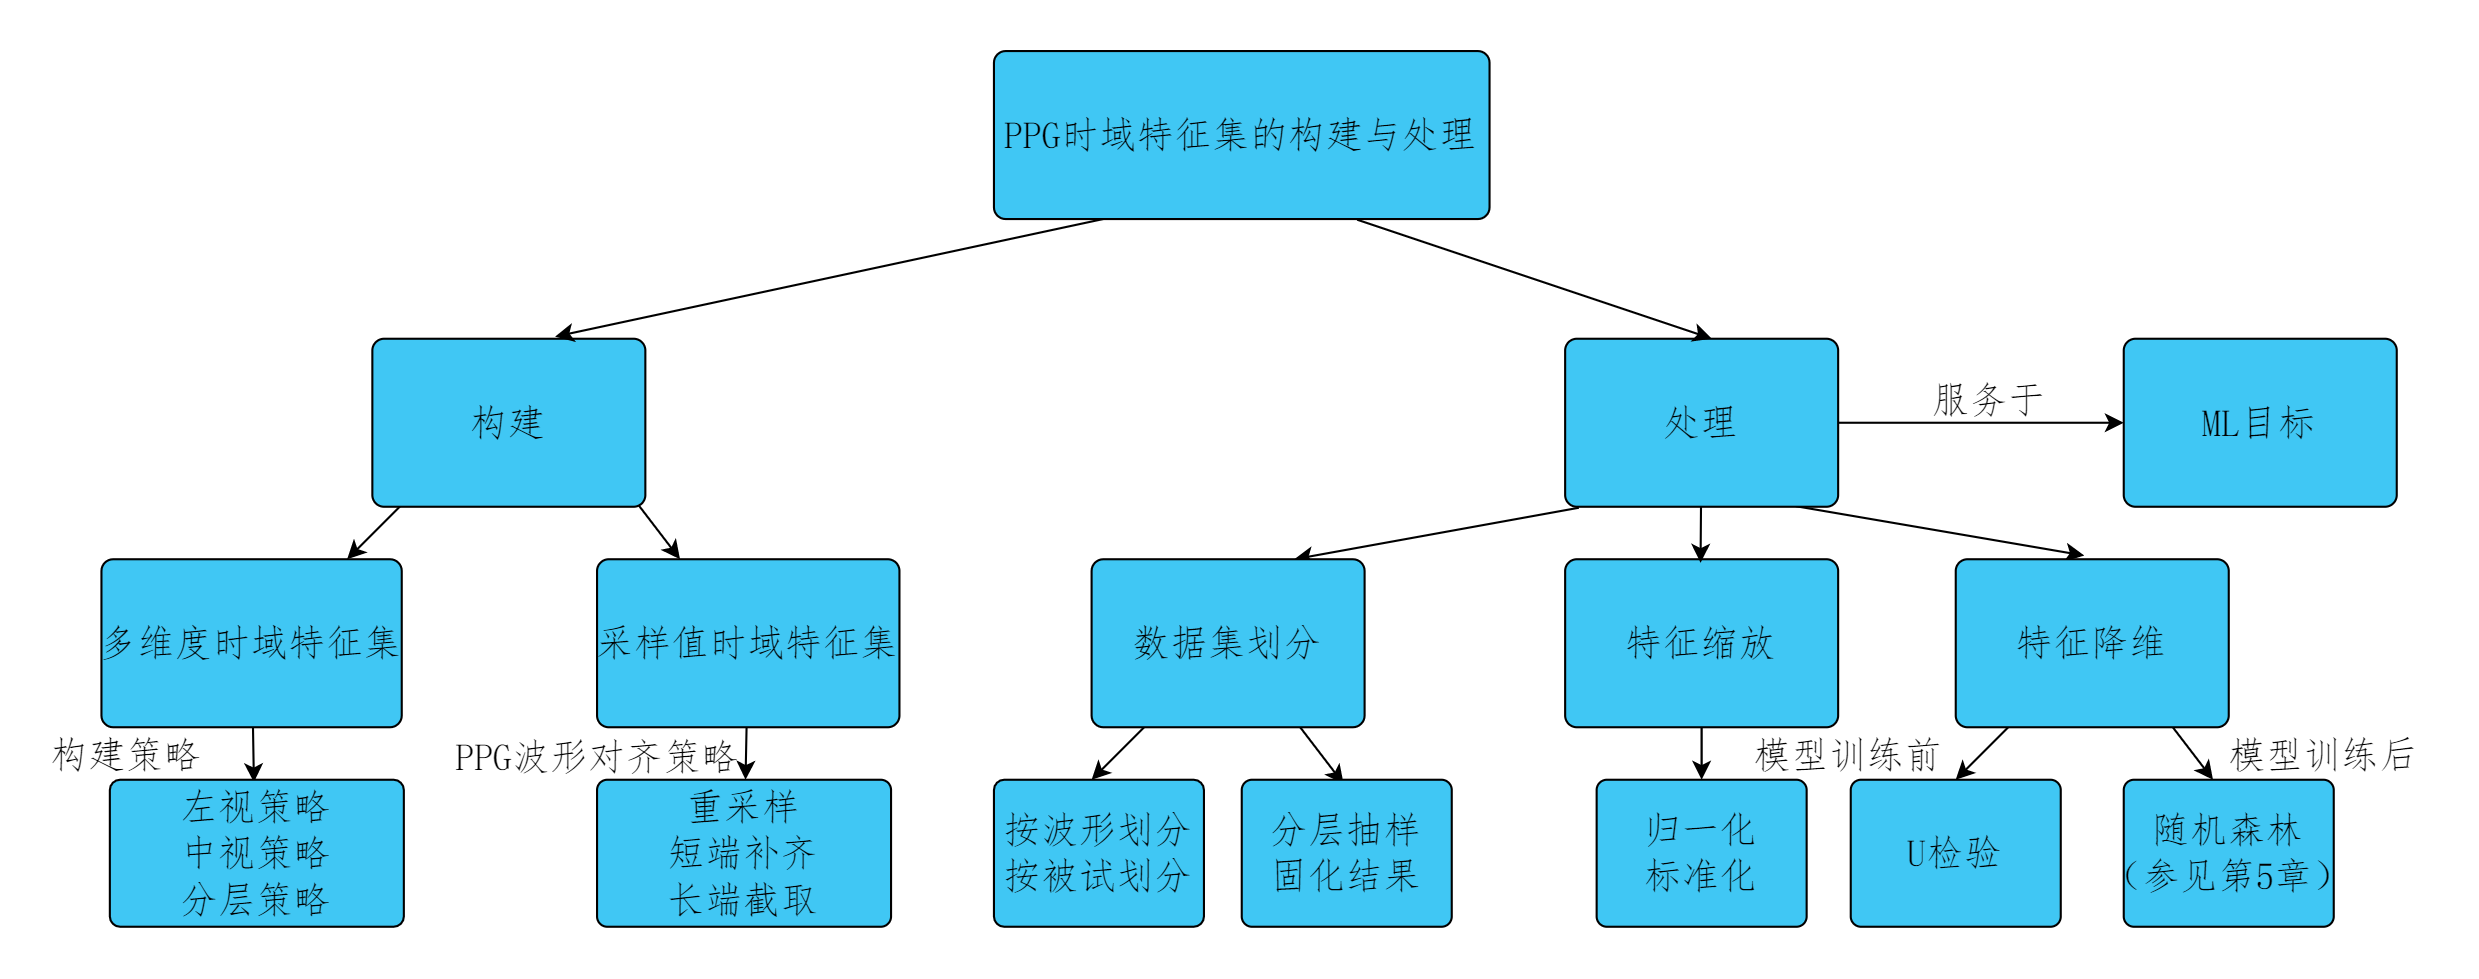
\includegraphics[width=0.9\linewidth]{features/frameworks4}
  \caption{\label{fig:frameworks4}第四章研究内容框架图}
\end{figure}

\section{脉搏波的新型时域特征参数设计}
本研究结合PPG形态特点,设计了多种新型时域特征参数,从时长、角度、斜率、弧度、弧长与面积等多个角度对PPG的形态特征进行描述,并提出了脉搏波波形特征描述向量的概念。
此外,也提出了三种可描述多个PPG波形间的差异的时域特征参数。

\subsection{新型时域特征的设计基础}

第二章已经介绍过,PPG的上升支是由于心脏收缩致使血液开始进入主动脉,并使血管壁扩张,最终导致动脉血压快速上升而形成的\cite{PPGYY}。该过程非常迅速,导致上升支大多较为陡峭,从形态上来看,PPG信号的上升支通常较下降支更为简单\cite{PPGYY,Chen2021}。
因此,对PPG的描述可着重聚焦于PPG的下降支,如\autoref{fig:ppg_roads}所示。
\begin{figure}[htbp]
  \centering
  \subfigure[\label{fig:pulsecontrast}同一被试的PPG的原始波形对比图]{
    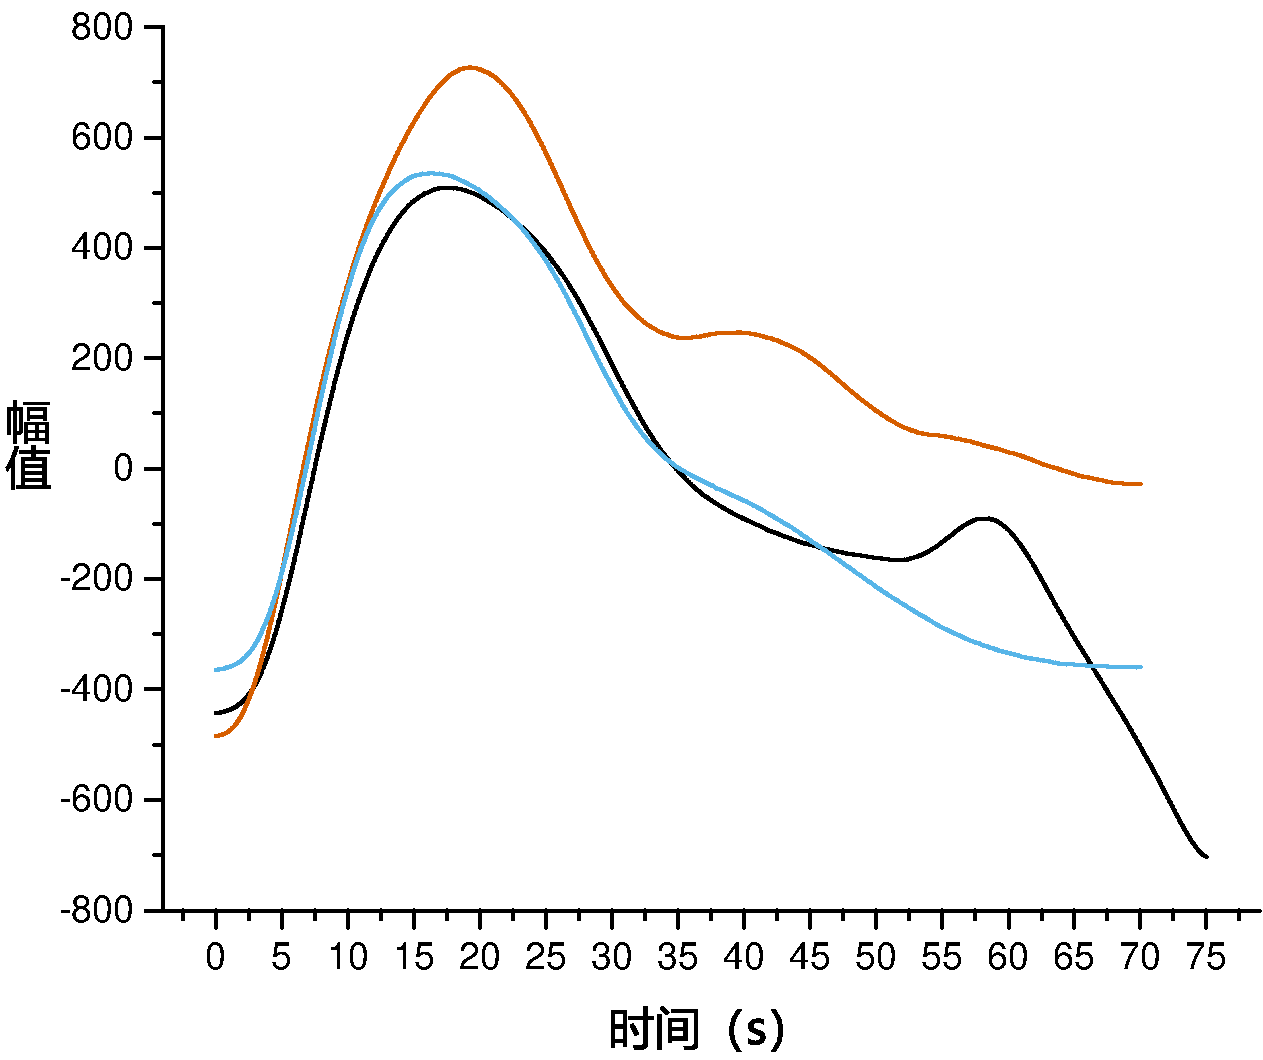
\includegraphics[width=6cm]{features/pulsecontrast}
  }
  \quad
  \subfigure[\label{fig:road}同一被试的PPG的下降支波形对比图]{
    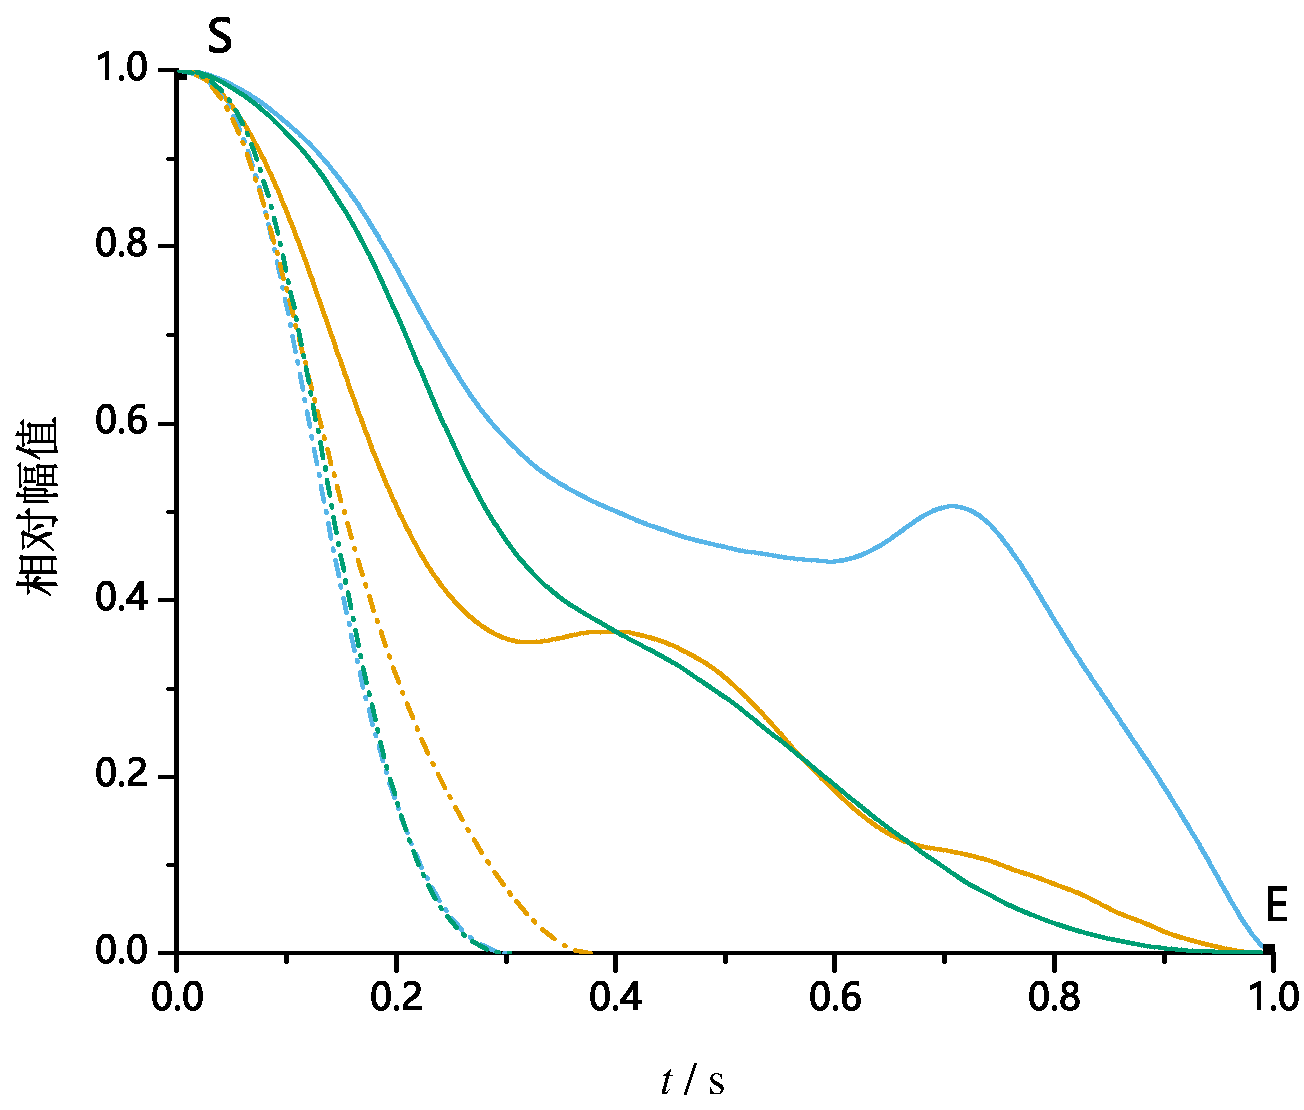
\includegraphics[width=6cm]{features/road}
  }
  \caption{\label{fig:ppg_roads}PPG波形及PPG下降支对比图}
\end{figure}

在图\autoref{fig:pulsecontrast}中,同一被试的三个PPG波形用不同颜色进行了区分对比,可以发现三个波形在重博的显著程度、持续时长及幅值大小等方面均存在着差异。
而图\autoref{fig:road}则对比了图\autoref{fig:pulsecontrast}中波形的下降支,其中,波形的下降支均进行了双向归一化处理。

由信号的采样定理可知,对PPG波形下降支的描述可通过对下降支上一系列点的描述来完成。不失一般性,若将下降支的起点坐标与终点坐标分别设置为$S$$(0,1)$与$E$$(1,0)$,
对于下降支上任意一点$P$,可以用原点$O$坐标$(0,0)$与路径始末点坐标$S$、$E$等为基本参照点,以及$P$
在X轴、Y轴上的投射点$P_x$、$P_y$等衍生参照点对该点进行描述,如\autoref{fig:point}所示,而对PPG上升支的描述与此过程类似。
上述过程中涉及的可用指标具体如\autoref{tab:pointsdesc}所示,部分参数指标的归一化/类归一化的无量纲形式也在\autoref{tab:pointsdesc}中进行了说明。

\begin{figure}[htbp]
  \centering
  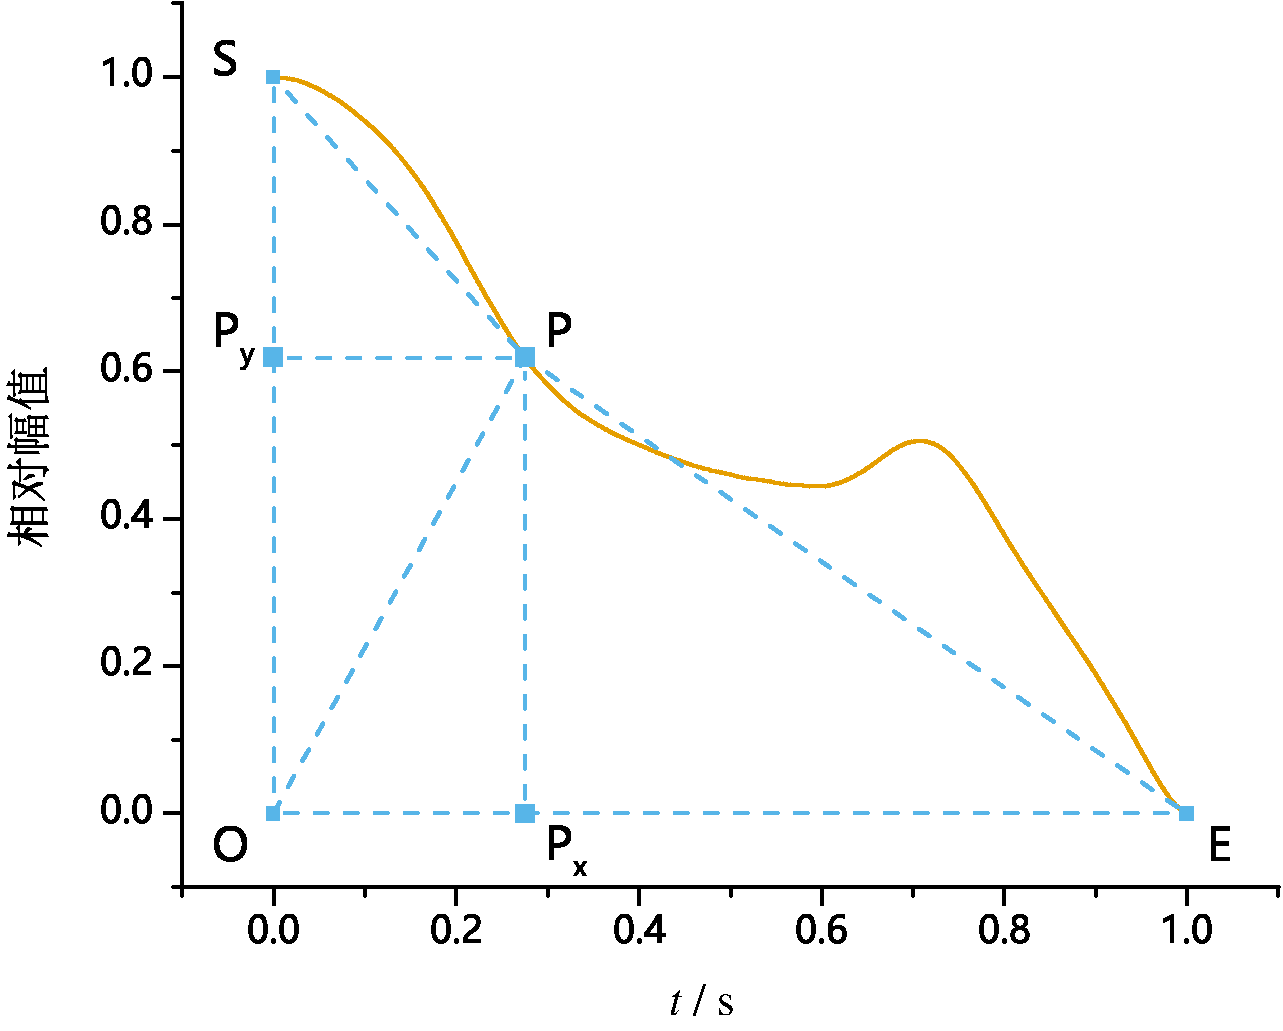
\includegraphics[width=.6\linewidth]{features/point}
  \caption{\label{fig:point}PPG波形下降支上任意点的描述示意图}
\end{figure}

\vspace{-1em}
\begin{center}
    \zihao{-5}
    \begin{longtable}{m{0.6cm}<{\centering}m{1.5cm}<{\centering}m{3.2cm}<{\centering}m{3cm}<{\centering}m{3.2cm}<{\centering}m{3cm}<{\centering}}
		\caption{PPG波形上任意一点的描述指标}\\
		\label{tab:pointsdesc}\\
		\topline
        \colorhead & & \multicolumn{2}{c}{\textbf{原始数值表达}} & \multicolumn{2}{c}{\textbf{归一化表达}} \\
        \colorhead \multirow{-2}{*}{\textbf{序号}}&\multirow{-2}{*}{\textbf{参数类型}}  & 物理意义 & 表达式或公式 & 物理意义 & 表达式或公式 \\
        \midline
        \endfirsthead
        \caption[]{(续)}\\
        \topline
        \colorhead   & & \multicolumn{2}{c}{\textbf{原始数值表达}} & \multicolumn{2}{c}{\textbf{归一化表达}} \\
        \colorhead \multirow{-2}{*}{\textbf{序号}}& \multirow{-2}{*}{\textbf{参数类型}}  & 物理意义 & 表达式或公式 & 物理意义 & 表达式或公式 \\
        \midline
        \endhead 
        \midline
        \endfoot
        \bottomline
        \endlastfoot
        \colorrowa 1 &                             & Y轴方向下降高度           &   $SP_y$      &  Y轴方向下降比例     & $ \displaystyle \frac{SP_y}{OS}$ \\
        \colorrowa 2 &                             & P点高度                  &   $OP_y$       &    P点高度与波峰比值   & $\displaystyle \frac{OP_y}{OS}$ \\
        \colorrowa 3 &                             & 从S点到P点所用时间        &    $OP_x$   &      起点至P点所用时间与下降支总时长比值 & $\displaystyle \frac{OP_x}{OE}$ \\
        \colorrowa 4 &                             & 从P点到E点所用时间        &    $EP_x$   &      P点至终点E所用时间与下降支总时长比值 & $\displaystyle \frac{EP_x}{OE}$ \\
        \colorrowa 5 &                             & OP两点间几何距离        &    $OP$   &  OP两点距离与SE两点距离之比     & $\displaystyle \frac{OP}{SE}$ \\
        \colorrowa 6 &                             & SP两点间几何距离        &    $SP$   &  SP两点距离与SE两点距离之比     & $\displaystyle \frac{SP}{SE}$ \\
        \colorrowa 7 & \multirow{-7}*{线段}         & PE两点间几何距离        &    $PE$   &  PE两点距离与SE两点距离之比     & $\displaystyle \frac{PE}{SE}$ \\
        \colorrowc 8 &                             &  SP两点间曲线弧长     &  $\displaystyle L_{\overset{\frown}{SP}}$     &     SP两点间曲线弧长与SE两点直线距离之比  & $\displaystyle \frac{L_{\overset{\frown}{SP}}}{SE}$ \\
        \colorrowc 9 & \multirow{-2}*{曲线长度} &  PE两点间曲线弧长   &   $\displaystyle L_{\overset{\frown}{PE}}$    &    PE两点间曲线弧长与SE两点直线距离之比  &  $\displaystyle \frac{L_{\overset{\frown}{PE}}}{SE}$\\
        \colorrowa 10 &                             &  线段SP的斜率     &  $\displaystyle -\frac{SP_y}{PP_y}$     &   /    &  /  \\
        \colorrowa 11 &                             &  线段PE的斜率     &   $\displaystyle -\frac{P_yP_x}{EP_x}$    &    /  &  /   \\
        \colorrowa 12 & \multirow{-3}*{斜率}        &  线段OP的斜率    &    $\displaystyle \frac{PP_y}{PP_x}$   &    /   &  /     \\
        \colorrowc 13 &                             &  $\angle SPP_y$的弧度      & $\displaystyle \arctan(\frac{SP_y}{PP_y})$     &    /  &  /   \\
        \colorrowc 14 &                             &   $\angle POE$的弧度    &  $\displaystyle \arctan(\frac{P_yP_x}{EP_x})$      &    /  &  /   \\
        \colorrowc 15 & \multirow{-3}*{\tabincell{c}{角度\\(弧度)}}&   $\angle PEO$的弧度   &  $\displaystyle \arctan(\frac{PP_y}{PP_x})$         &    /  &  /   \\
        \colorrowa 16 &                             &    坐标轴、曲线与$PP_y$以上围成的面积   &  $\displaystyle \int_{P_y}^{S}{P(t)dy} $     &   前述面积与整体面积之比    & $\displaystyle \frac{\int_{P_y}^{S}{P(t)dy}}{\int_O^E{P(t)dx}}$ \\
        \colorrowa 17 & 面积                            &   坐标轴、曲线与$OP$以左围成的面积   &    $\displaystyle \int_{O}^{P_x}{P(t)dx}-S_{\triangle OPP_x}$   &  前述面积与整体面积之比     & $\displaystyle \frac{\int_{O}^{P_x}{P(t)dx}-S_{\triangle OPP_x}}{\int_O^E{P(t)dx}}$ \\
        \colorrowa 18 &                             &   坐标轴、曲线与$PP_x$以左围成的面积   &   $\displaystyle \int_{O}^{P_x}{P(t)dx}$    &  前述面积与整体面积之比     & $\displaystyle \frac{\int_{O}^{P_x}{P(t)dx}}{\int_O^E{P(t)dx}}$ \\
        \colorrowa 19 &         &    曲线与$SP$围成的面积   &   $\displaystyle \int_{P_y}^{S}{P(t)dy}-S_{\triangle SPP_y} $    &   /    &  /\\
	\end{longtable}
\end{center}
\vspace{-0.8cm}

结合\autoref{tab:pointsdesc}与\autoref{fig:point}可知,在PPG波形上任意确定一点$P$,与$P$关联的线段指标、曲线长度指标、斜率指标、弧度指标及面积指标等都可以得到确定并有与之对应的唯一数值。
反之,若以\autoref{tab:pointsdesc}中某一指标为基准,并在该指标的值域内选定一具体数值,则在PPG波形上也可以确定与之对应的参考点$P'$,进一步可由$P'$得到其他描述参数的具体数值。

\subsection{脉搏波波形特征描述向量}

对于\autoref{tab:pointsdesc}的任意特征而言,若按照上一小节的方法在PPG波形上确定多个描述点,即可得到同一特征的多个有关联性的数值。本研究将这些有关联性的数值称为脉搏波特征描述向量(photoplethysmographic feature vector,PPGFV)
\begin{equation}
  \label{equ:featurevector}
  \boldsymbol {V_n}=[v_0,v_1,\cdots,v_{n-1}]
\end{equation}
其中,$v$对应\autoref{tab:pointsdesc}中的具体特征,$n$是向量的维数,可以视情况人工设定。

PPGFV最显著的特点在于用一组相互联系的数值来量化描述PPG波形,这与第三章中介绍的诸多通过单一数值描述PPG波形的时域特征参数迥然不同。
若某一PPG波形的采样点数为$N$,则该波形可以视为$n=N$的特殊PPFV;同理,当该波形经插值处理后的结果可以看成$n>N$的PPFV;
而使用第三章中介绍的时域特征描述该波形时,这些参数均可视为$n=1$的PPFV。

因此,PPFV对波形的描述能力随着其向量维数的增加而增强;而对波形的抽象与概括能力随之削弱。
这一现象可以用信息论中的编码理论进行解释,在信源原始符号不变的情况下,
增加变换编码的输出符号长度可以提高系统在通讯过程中的信息传输能力\cite{Zhao2017}。
从这个角度理解,PPGFV是在变换编码背景下一种编码长度与信息描述能力的折中与妥协。

\subsection{脉搏波波形间差异的描述特征}
上文介绍的PPG时域特征参数均是对一个完整的PPG波形进行量化描述,但在某些情景下,多个PPG波形间的差异可能更需要被研究者们关注。对同一被试而言,这种波形间的差异可以
称为PPG波形的紊乱程度,如\autoref{fig:diff_in_pulse}所示。

\begin{figure}[htbp]
  \centering
  \subfigure[\label{fig:dp0}实验组被试波形示意图]{
  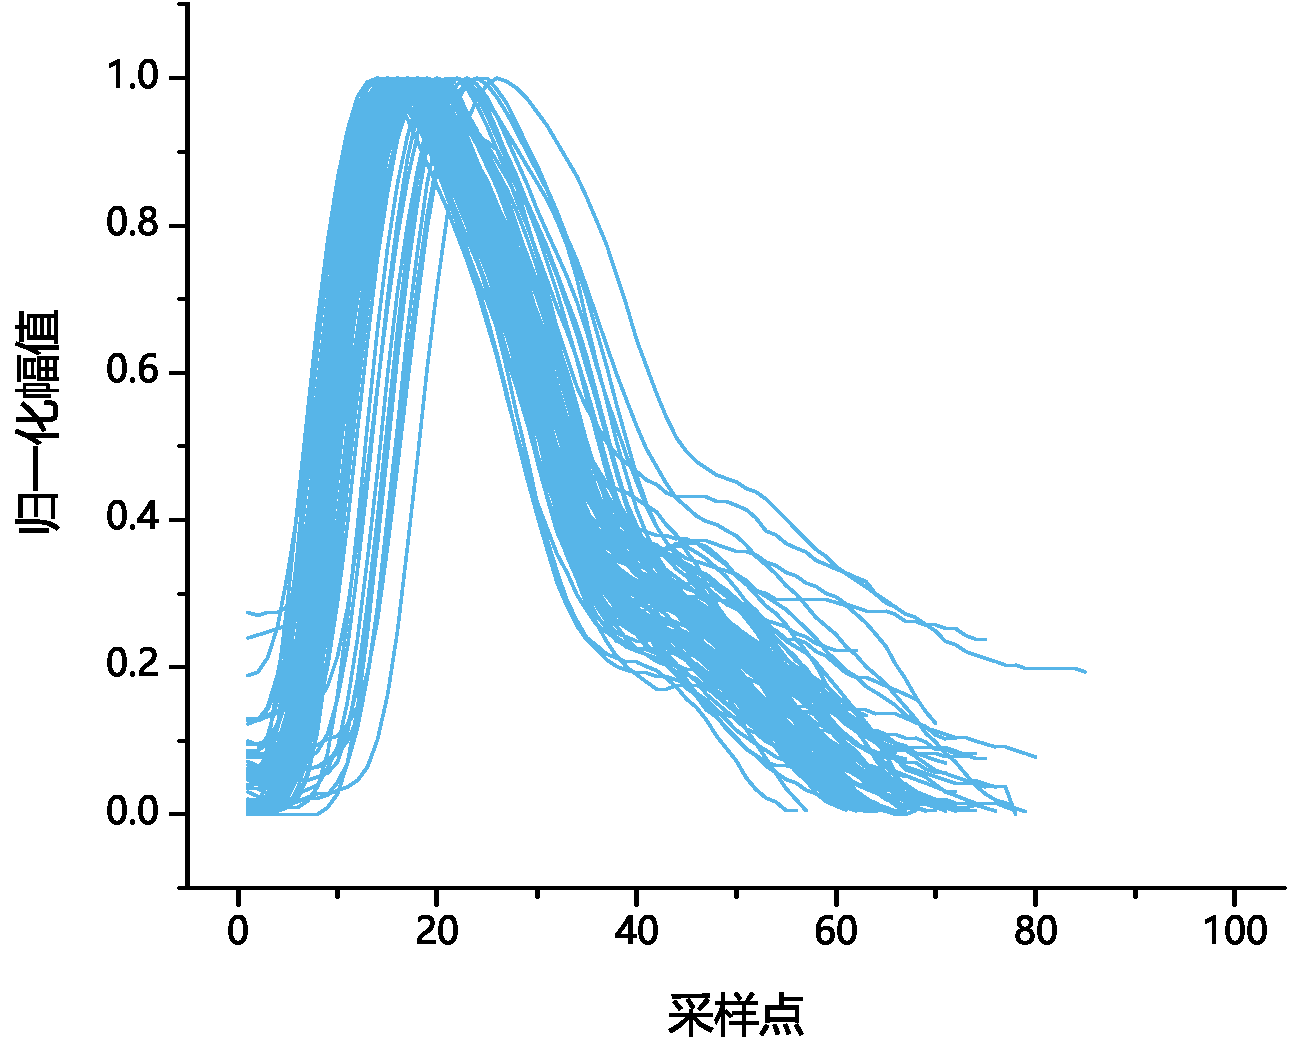
\includegraphics[width=6cm]{features/cmf}
  }
  \quad
  \subfigure[\label{fig:dp1}对照组被试波形示意图]{
    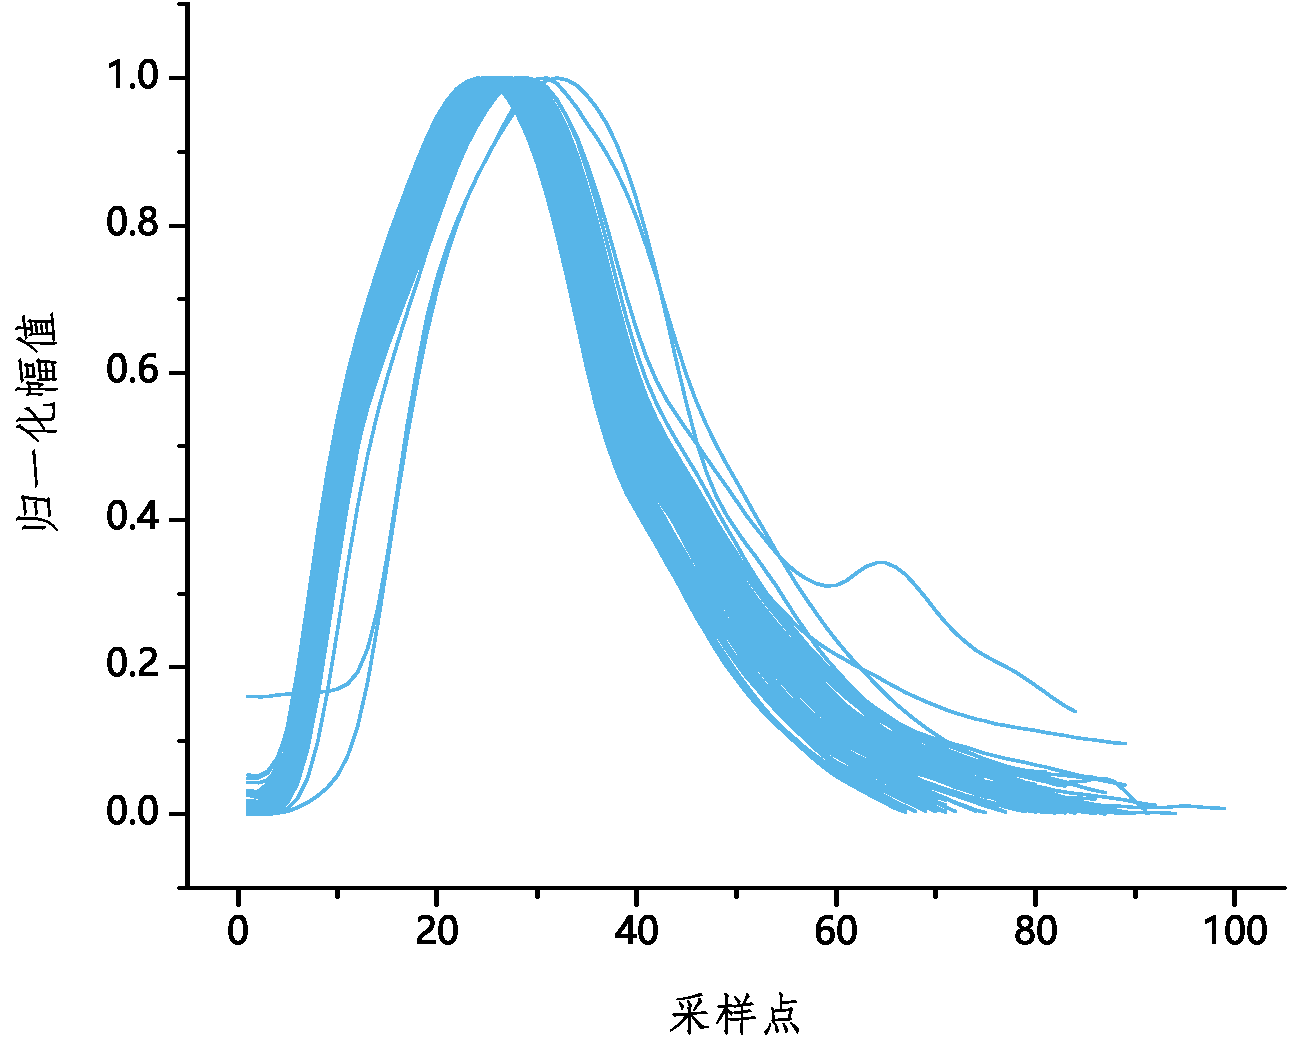
\includegraphics[width=6cm]{features/wjh}
  }
  \caption[脉搏波波形间的差异性]{\label{fig:diff_in_pulse}脉搏波波形间的差异性示意图}
\end{figure}

\autoref{fig:diff_in_pulse}对同一被试的所有PPG波形按起点进行了对齐,即使对同一被试而言,其波形的形态特征、波形时长同样存在一定的差异,而这些差异在不同的个体之间体现得更为明显。

因此,本小节提出通过相关系数、弗朗明歇距离与包络面积等三种时域参数量化描述脉搏波波形间的差异性。

一、相关系数

本研究将统计分析中衡量两个变量因素的密切程度的相关系数引入两个波形之间的“相似”程度的衡量中。

第三章中介绍过具有代表性的皮尔逊相关系数与斯皮尔曼相关系数。但斯皮尔曼相关系数在计算时必须对原始数据排序,会直接破坏PPG波形数据的有序性。
因此,本研究选取了皮尔逊相关系数$r_p$衡量波形间的相似性
\begin{equation}
    \label{equ:pearson2}
    r_p=\frac{\sum_{i=1}^n{(x_i- \mathop{x} \limits^-)(y_i- \mathop{y} \limits^-)}}{\sqrt{{\sum_{i=1}^n}{{(x_i- \mathop{x} \limits^-)^2\sum_{i=1}^n}{(y_i- \mathop{y} \limits^-)^2}}}}
\end{equation}

波形间相关系数值越大,两个PPG波形越“相似”。

二、弗朗明歇距离

弗朗明歇距离(Fréchet distance,FD)是最早由法国数学家Maurice René Fréchet于1906年提出的一种路径空间相似形描述方法\cite{Wien1994,Kaveh2013,GN2017,derohde2022}。

FD的完整数学定义如下,若将曲线视为其在定义域至度量空间的一种映射关系,即$[a,b]\rightarrow V$,
那么对曲线$f:[a,b]\rightarrow V$与曲线$g:[a',b']\rightarrow V$,两者的弗朗明歇距离为
\begin{equation}
    \label{equ:frechet distance}
    \delta_F(f,g)=\inf \max \limits_{\alpha,\beta \; t \in (0,1)} d(f(\alpha(t)), g(\beta(t)))
\end{equation}
其中,$\alpha$与$\beta$是满足能将$[0,1]$分别映射至$[a,b]$与$[a',b']$的任意连续非递减函数,$d$是$V$上的度量函数\cite{Wien1994}。
二维空间上的FD如\autoref{fig:frechet distance}所示。
\begin{figure}[htbp]
  \centering
  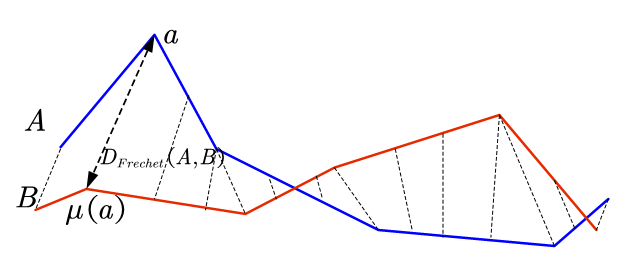
\includegraphics[width=.5\linewidth]{features/frechet_distance1}
  \caption{\label{fig:frechet distance}二维空间上的弗朗明歇距离示意图}
\end{figure}

对于两个PPG波形而言,此时的FD已经退化成在相同采样点的采样幅值之差的最大值,波形间的弗朗明歇距离值越小,两者越“相似”。

三、包络面积差

包络面积差(difference of envelope area ,DEA)是本研究提出的用以描述脉搏波间差异的原创指标,两个PPG波形的幅值差值的积分结果,如\autoref{fig:dea}所示。
\begin{equation}
    \label{equ:dea}
    \begin{aligned}
        \text{EDA} &= \int_{t_0}^{t_n}|P_f(t)-P_g(t)|dt\\
        &\approx \frac{\Delta t}{2} \sum_{i=0}^{n-1}{|(P_f(i)+P_f(i+1)-(P_g(i)+P_g(i+1))|}
    \end{aligned}
\end{equation}
\begin{figure}[htbp]
  \centering
  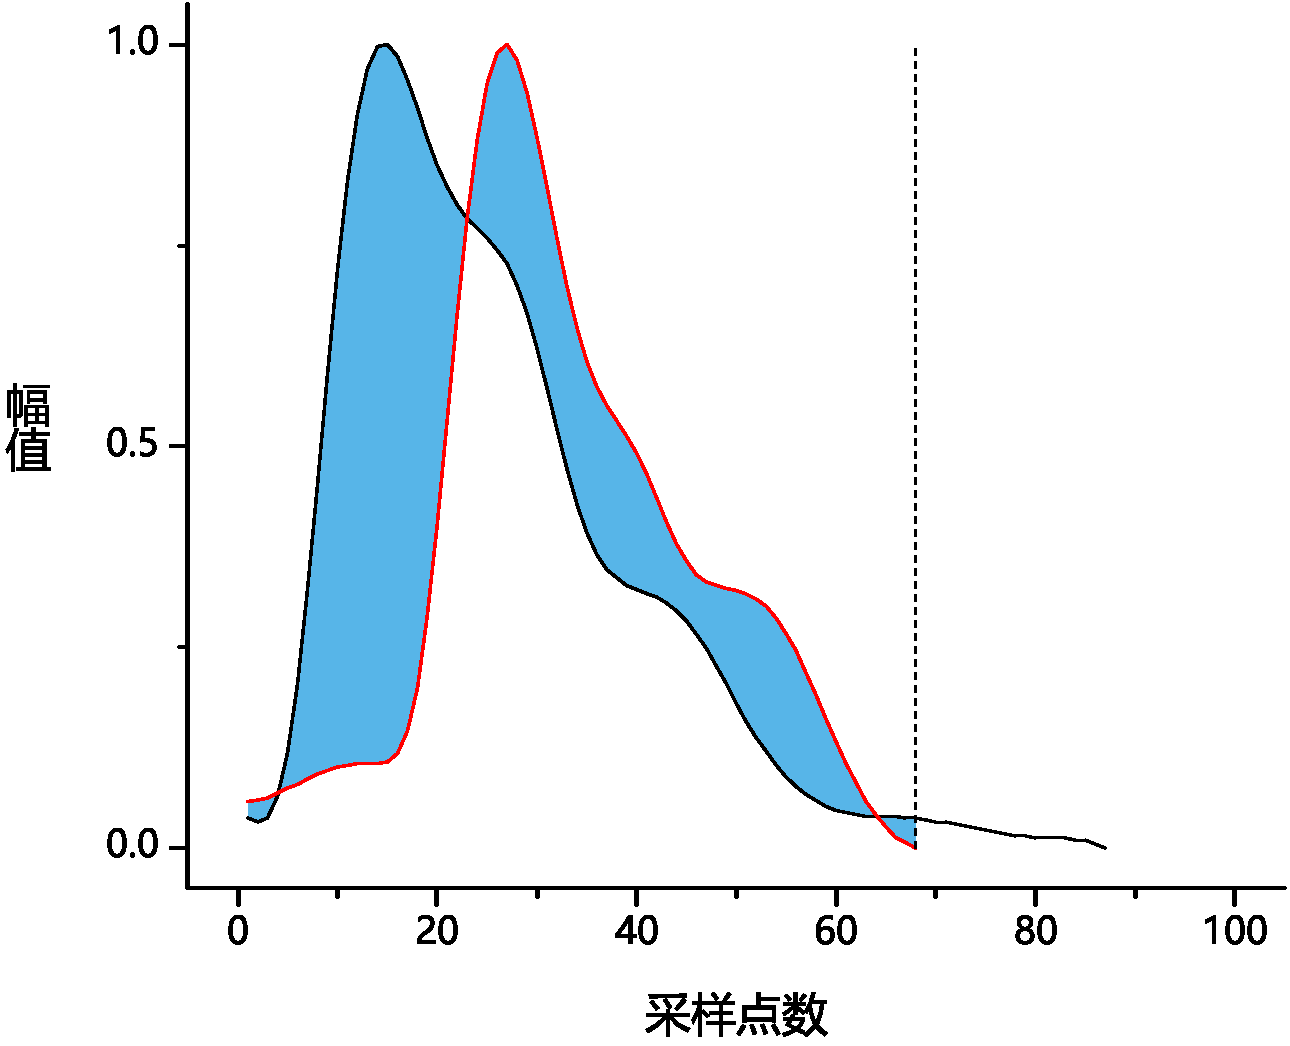
\includegraphics[width=0.6\linewidth]{features/dea0}
  \caption[包络面积差示意图]{\label{fig:dea}包络面积差示意图}
\end{figure}

两个波形间包络面积差值越小,两者越“相似”。

四、波形采样点对齐

上述三个描述波形间相似度(或差异度)的时域参数的计算都包含了一个隐藏的前置条件,即参与计算的两个波形的时间序列有着相等的采样点数。
而由于PPG信号本身的随机性,这样的条件在实际中几乎不可能被满足,如\autoref{fig:diff_in_pulse}与\autoref{fig:dea}所示\cite{Qiu2012,PPGYY,Ma2015}。
这也要求在计算这些参数时必须考虑波形的采样点数对齐问题。

本研究提出了将PPG波形对齐的三种处理策略,分别为重采样策略(resampling strategy, RS)、补齐策略(complementary strategies,CS)
与截取策略(interception strategy,IS)。为说明三种策略处理思路,下面以两个PPG波形的对齐处理过程为例,记这两个波形的原始采样数分别记为$m$、$n$且$m \neq n$,不失一般性,设$m>n$。

1、重采样策略(RS)

重采样策略通过信号的插值与抽取调整数据采样率,随后将两个PPG波形的采样点数调整至相同数值$n_r$。
若按RS将采样长度为$m$的波形调整至$n_r$,记$m$与$n_r$的最小公倍数为$p$,只需将原始数据均匀插值至$p$点,再按每$p/n_r$个点进行抽取即可。

2、补齐策略(CS)

补齐策略则是以采样点数为$m$的PPG波形为基准,对两一个波形在尾端直接进行补零处理,使两者的采样点均达到$n_c$($n_c=m$)。

3、截取策略(IS)

与补齐策略相反,截取策略会以采样点数为$n$的PPG波形为基准,舍弃掉另一个波形在$n$点以后的采样值,使两者的采样点均达到$n_i$($n_i=n$)。

将图\autoref{fig:dp0}中的被试数据分别按以上三种对齐策略处理,所得效果如\autoref{fig:no_pe2}所示。

\begin{figure}[htbp]
  \centering
  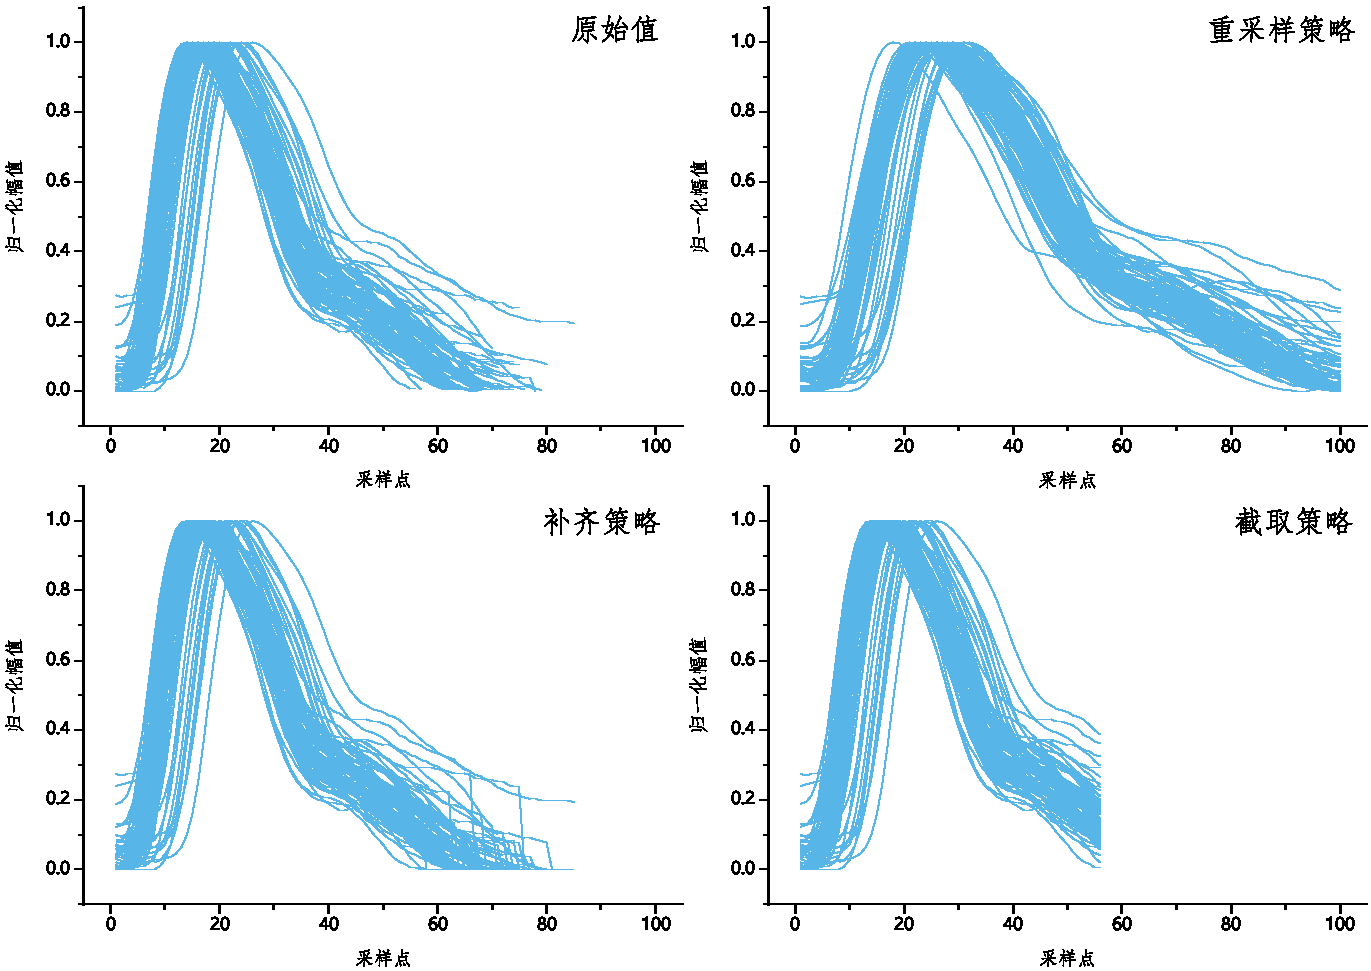
\includegraphics[width=0.75\linewidth]{features/alignment}
  \caption{\label{fig:no_pe2}同一被试PPG波形按三种对齐策略处理效果对比图}
\end{figure}

从\autoref{fig:no_pe2}可以看到,三种策略均可以完成PPG波形的对齐处理。但按截取策略处理时,出现了不可忽视的数据损失,因此截取策略在后续处理中被暂时弃用。

五、多个波形间的差异性描述

此前介绍的三种参数都是对两个波形间差异的描述,但对更多波形间差异的描述也可按照这种思路进行。

若需量化\autoref{fig:diff_in_pulse}所示$n$个波形间的整体差异性,可按排列组合的方法每次从$n$个波形间
选取两个波形,并用上述三种描述参数进行量化,得到3组描述数据,每组有$C_n^2$个具体数值。可按数理统计的一般方法,用这3组数据的平均值、方差、标准差、极值等指标对这$n$个
波形的差异进行整体性描述。

\section{脉搏波时域特征集的构建}
作为后续章节PE的ML模型的数据准备,本小节在前文新型时域特征的设计基础上,本小节完成了\textbf{脉搏波多维度时域特征集}(photoplethysmographic multidimensional time-domain feature set,PPGMTFS)
与\textbf{脉搏波采样序列时域特征集}(photoplethysmographic sampling series time-domain feature set,PPGSSTFS)的构建工作。

由于设计理念不同,本论文并未将以上两个特征集进行合并或交叉处理,这两个特征集合各自被\textbf{独立地}用作后续PE识别分析阶段的输入数据。
而在预研究中,4.2.3小节提出的PPG波形间时域特征参数未能构建出效果较好的PE识别模型,故将其未作为后续分析的输入使用。

\subsection{脉搏波多维度时域特征集}

本小节是在4.2.1与4.2.2小节的基础上,按照一定的标准,在PPG波形上确定多个基准参考点,得到与这些基准点关联的一系列基于线段、曲线长度、斜率、弧度及面积等多维度脉搏波特征描述向量(PPGFV)。

一、基准点的确定策略

在PPG波形上选取并确定基准点的过程,是通过PPGFV对PPG进行描述的关键。本研究共使用了三种策略,分别为左视策略(left-view strategy,LVS)、中视策略(middle-view strategy,MVS)与分层策略(hierarchical strategy,HS)。
这三种策略的概念图如\autoref{fig:all_views}所示。

1、左视策略(LVS)

左视策略以PPG上升支起点为原点$T$,同时将PPG波峰设为$P$,将线段$TP$与水平基线$TT'$所构成的夹角$\angle PTT'$等分成若干份。这些等分线与PPG的交点${Q'}_i$被确定为参考基准点,这一过程如图\autoref{fig:lv}所示。

2、中视策略(MVS)

中视策略以PPG波峰$P$在水平线$TT'$上的映射点$O$为原点,将线段$OP$与水平基线构成的两个夹角$\angle POT$与$\angle POT'$等分成若干份。将这些等分线与PPG的上升支、下降支的交点计为参考基准点${Q'}_i$,这一过程如图\autoref{fig:mv}所示。

3、分层策略(HS)

分层策略将PPG波峰$P$在水平线$TT'$上的映射点计为$O$,作线段$OP$的水平垂线将$OP$等分为若干份。将这些等分线与PPG的上升支、下降支的交点计为参考基准点${Q'}_i$,这一过程如图\autoref{fig:hv}所示。

\begin{figure}[htbp]
  \centering
  \subfigure[\label{fig:lv}左视类指标示意图]{
  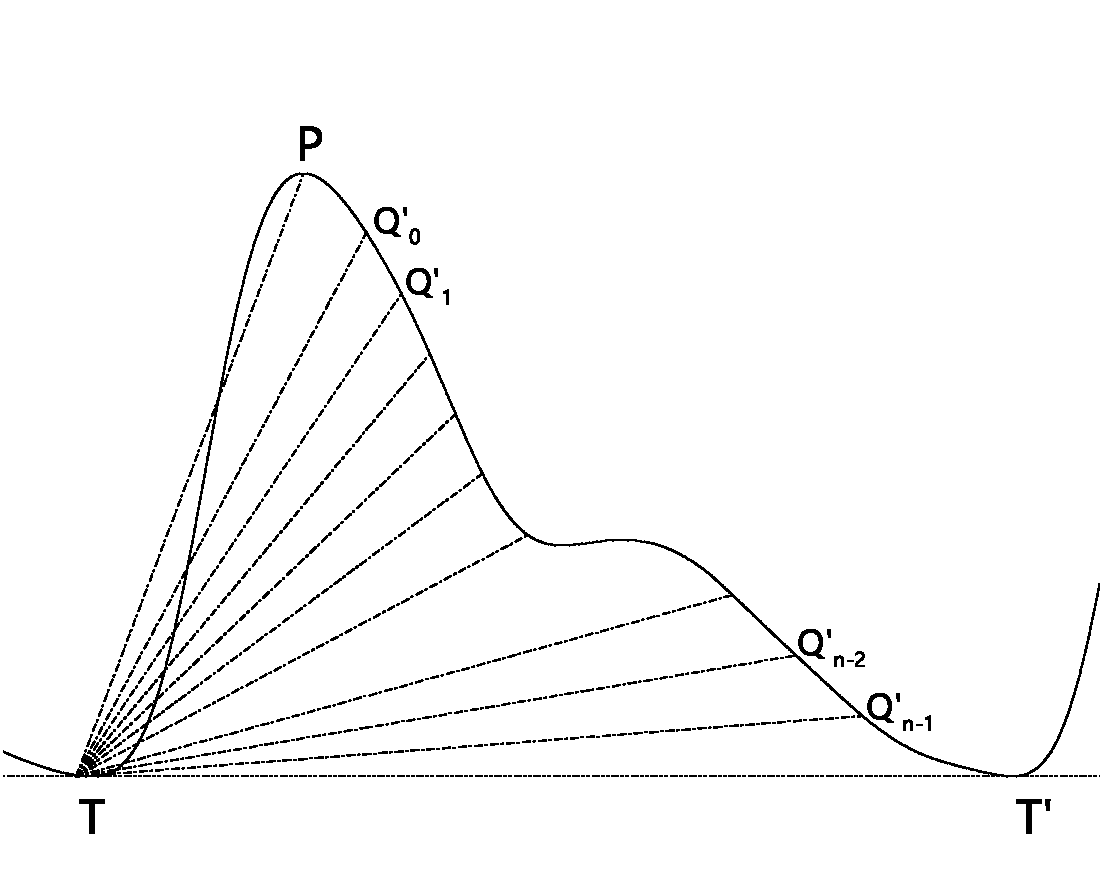
\includegraphics[width=6cm]{features/lv}
  }
  \quad
  \subfigure[\label{fig:mv}中视类指标示意图]{
  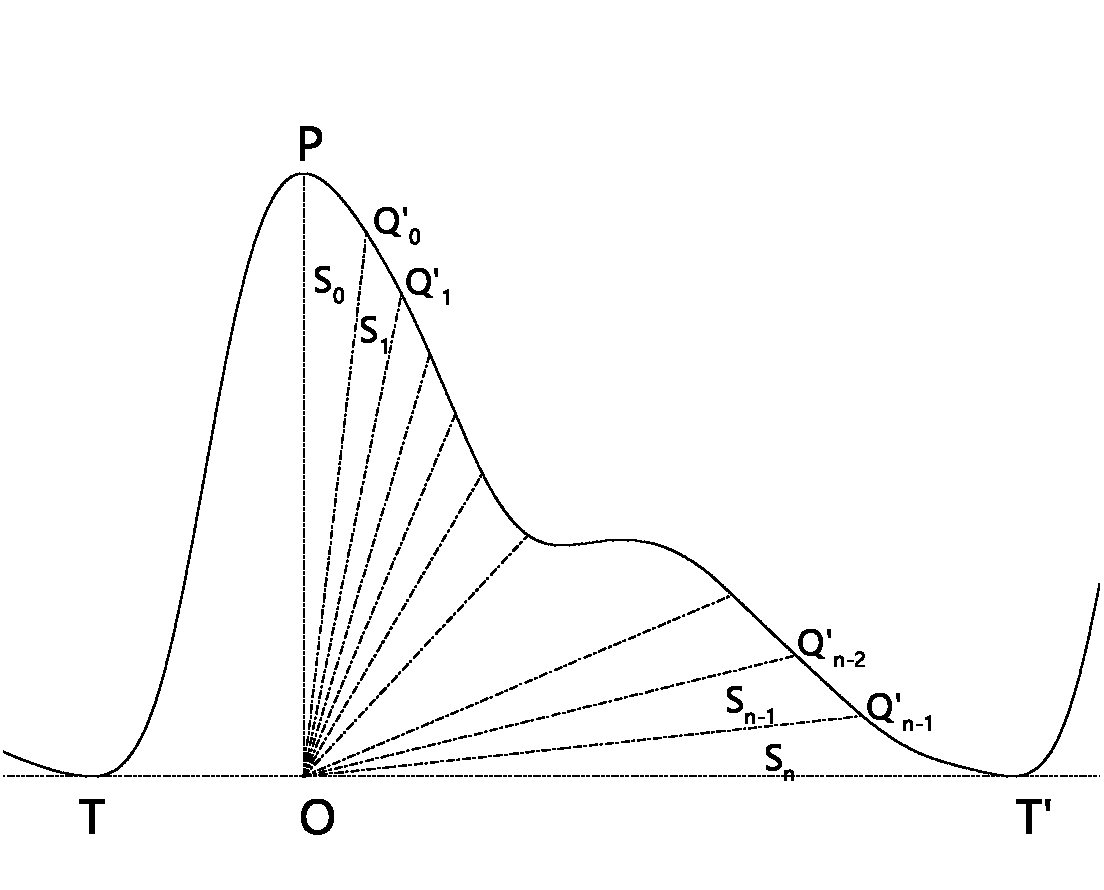
\includegraphics[width=6cm]{features/mv}
  }
  \quad
  \subfigure[\label{fig:hv}分层类指标示意图]{
  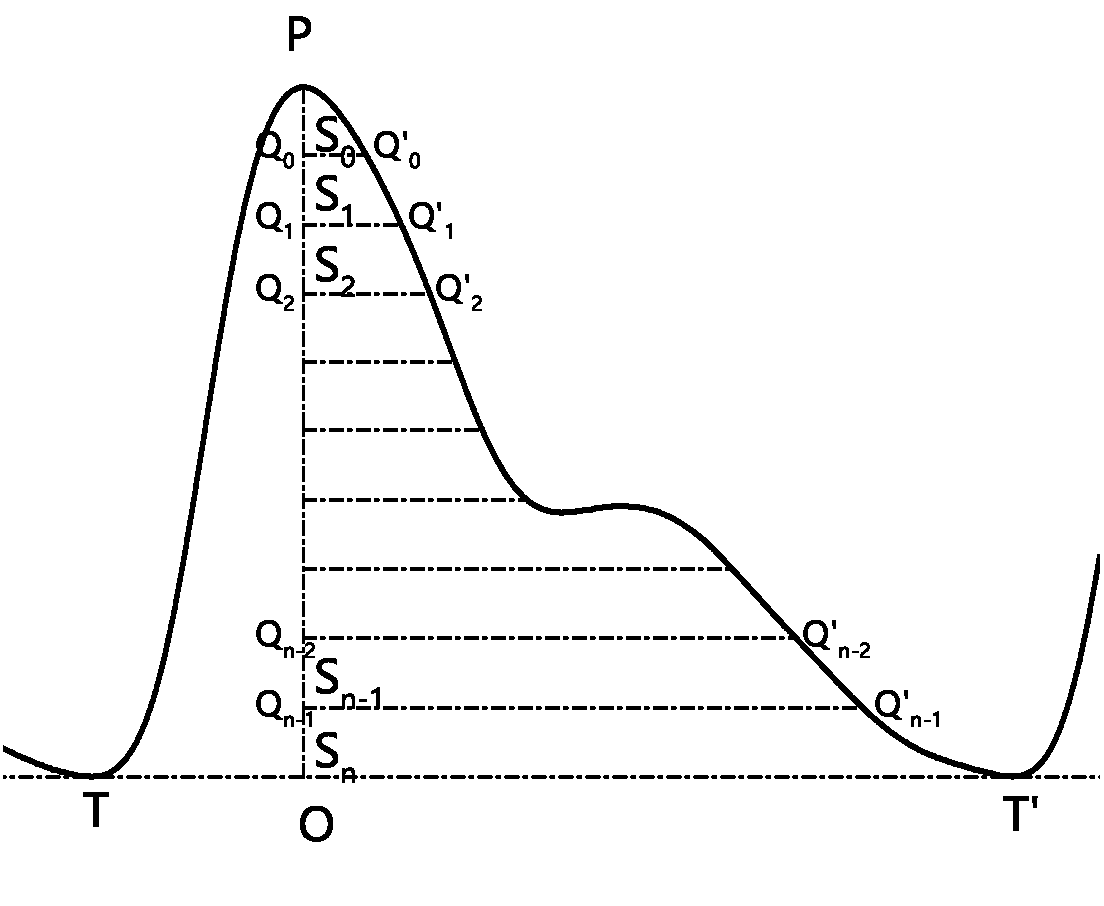
\includegraphics[width=6cm]{features/hv}
  }
  \caption{\label{fig:all_views}确定基准点的三种策略示意图}
\end{figure}

二、基准点的维数

选取基准点的标准确定之后,另一个需要确定的问题时基准点的维数问题。
在4.2.2小节已经阐述过,脉搏波特征描述向量(PPGFV)是在变换编码背景下一种编码长度与信息描述能力的折中与妥协。

本研究通过前期预研究,最终确定了上述三种确定基准点策略下的具体维数。
其中,分层策略的维数为10;而左视策略与中视策略下的基准点确定都涉及了角度处理(需要对$\pi$进行处理),为简化计算过程,其维数都被确定为12。

故在分层策略下的新型时域特征的下标为0至9,左视策略与中视策略下的新型时域特征的下标为0至11。其中,下标数值越小,代表该特征在对应的PPG波形中越接近波峰;反之,则越远离波峰(更加接近波形的起点或终点)。

三、脉搏波多维度时域特征集具体包含特征

由于在计算PPG的时域特征之前,需要将PPG波形进行了标准化处理,使其幅值被调整缩放至[0,1000]区间内。
在此过程中,PPG波形的上升支与下降支分别按3.4.4小节中的线性变换思想进行了处理。
而线性变换过程中的截距与斜率本身也是多维度特征的一种,因此,本研究也这4个参数作为第4类标准化参数,纳入进PPG多维度时域特征集中。

\autoref{tab:allfeatures}中展示了上述标准化参数与经由左视策略、中视策略与分层策略确定得到的多维度时域特征。
\vspace{2em}
\begin{center}
  \zihao{-5}
  \begin{longtable}{m{1cm}<{\centering}m{1.4cm}<{\centering}m{3.3cm}<{\centering}m{1.5cm}<{\centering}m{7.5cm}<{\centering}}
    \caption{PPG多维度时域特征集合}\\
    \label{tab:allfeatures}\\
        \topline
        \colorhead \textbf{序号} & \textbf{类别}&\textbf{特征名称}&\textbf{缩写符号}&\textbf{物理意义}\\
        \midline
        \endfirsthead
        \caption[]{(续)}\\
        \midline
        \colorhead \textbf{序号} & \textbf{类别}&\textbf{特征名称}&\textbf{缩写符号}&\textbf{物理意义}\\
        \midline
        \endhead 
        \midline
        \endfoot
        \bottomline
        \endlastfoot
        \colorrowc 1 & &     上升支标准化斜率 & STDKR & 标准化PPG上升支波形至[0-1000]时使用的斜率 \\
        \colorrowc 2 & &     上升支标准化截距 & STDBR & 标准化PPG上升支波形至[0-1000]时使用的截距 \\
        \colorrowc 3 & &     下降支标准化斜率& STDKF & 标准化PPG下降支波形至[0-1000]时使用的斜率 \\
        \colorrowc 4 & \multirow{-4}*{标准化指标}   &  下降支标准化截距 & STDBF & 标准化PPG上升支波形至[0-1000]时使用的截距 \\
        \colorrowa 5 & &     左视斜率    &   LVS    &   各等分线所对应的直线斜率   \\
        \colorrowa 6 & &     左视上升支交点坐标 & LVLR & 等分线与PPG波形上升支交点横坐标 \\
        \colorrowa 7 & &     左视下降支交点坐标 & LVLF & 等分线与PPG波形下降支交点横坐标 \\
        \colorrowa 8 & &     左视上升支交点距离 & LVRR & 等分线与PPG波形上升支交点与波形起点距离 \\
        \colorrowa 9 & &     左视下降支交点距离 & LVRF & 等分线与PPG波形下降支交点与波形起点距离 \\
        \colorrowa 10 & &     左视交点坐标差 & LVD & 左视上升支交点坐标与左视下降支交点坐标之差 \\
        \colorrowa 11 & &     左视上升支弧长 & LVALR & PPG波形上升支被等分线分割的各区间弧长 \\
        \colorrowa 12 & \multirow{-8}*{左视策略} & 左视下降支弧长 & LVALF & PPG波形下降支被等分线分割的各区间弧长 \\
        \colorrowc 13 & &     中视上升支交点坐标 & CVLR & 等分线与PPG波形上升支交点横坐标 \\
        \colorrowc 14 & &     中视下降支交点坐标 & CVLF & 等分线与PPG波形下降支交点横坐标 \\
        \colorrowc 15 & &     中视上升支交点距离 & CVRR & 等分线与PPG波形上升支交点与峰值水平映射点距离 \\
        \colorrowc 16 & &     中视下降支交点距离 & CVRF & 等分线与PPG波形下降支交点与峰值水平映射点距离 \\
        \colorrowc 17 & &     中视交点坐标差 & CVD & 中视上升支交点坐标与中视下降支交点坐标之差 \\
        \colorrowc 18 & &     中视上升支弧长 & CVALR & PPG波形上升支被等分线分割的各区间弧长 \\
        \colorrowc 19 & &     中视下降支弧长 & CVALF & PPG波形下降支被等分线分割的各区间弧长 \\
        \colorrowc 20 & &     中视上升支面积 & CVAR & PPG波形上升支被等分线分割的各区域面积 \\
        \colorrowc 21 & \multirow{-9}*{中视策略} &     中视下降支面积 & CVAF & PPG波形下降支被等分线分割的各区域面积 \\
        \colorrowa 22 & &     分层上升支交点坐标 & SVLR & 等分线与PPG波形上升支交点横坐标 \\
        \colorrowa 23 & &     分层下降支交点坐标 & SVLF & 等分线与PPG波形下降支交点横坐标 \\
        \colorrowa 24 & &     分层上升支面积 & SVAR & PPG波形上升支被等分线分割的各区域面积 \\
        \colorrowa 25 & &     分层下降支面积 & SVAF & PPG波形下降支被等分线分割的各区域面积 \\
        \colorrowa 26 & &     分层面积 & SVAT & PPG波形整体被等分线分割的各区域面积 \\
        \colorrowa 27 & &     分层上升支交点距离 & SVRR & 等分线与PPG波形上升支交点与峰值水平映射点距离 \\
        \colorrowa 28 & &     分层下降支交点距离 & SVRF & 等分线与PPG波形下降支交点与峰值水平映射点距离 \\
        \colorrowa 29 & &     分层交点坐标差 & SVD &  分层上升支交点坐标与分层下降支交点坐标之差\\
        \colorrowa 30 & &     分层上升支弧长 & SVALR & PPG波形上升支被等分线分割的各区间弧长 \\
        \colorrowa 31 & &     分层下降支弧长 & SVALF & PPG波形下降支被等分线分割的各区间弧长 \\
        \colorrowa 32 & &     分层上升支斜率 & SVSR & \tabincell{c}{等分线与PPG波形上升支交点与PPG\\峰值水平映射点所形成直线的斜率}\\
        \colorrowa 33 & \multirow{-12}*{分层策略} & 分层下降支斜率 & SVSF & \tabincell{c}{等分线与PPG波形下降支交点与PPG\\峰值水平映射点所形成直线的斜率} \\
  \end{longtable}
\end{center}
\vspace{-1.2cm} 

在\autoref{tab:allfeatures}中,左视策略下确定了8种脉搏波特征描述向量(PPGFV),中视策略下
确定了9种PPGFV,分层策略下确定了12种PPGFV。而上小节已经对各策略下的维数进行过说明,
故PPG多维度时域特征集一共包含$4+12 \times 8+ 12 \times 9 + 10 \times 12$=328种特征值。对这328个特征的取值范围进行分析,可发现部分数值始终为0(通常这是由于该特征总对应着PPG波形的起点),
将这部分特征剔除后,脉搏波多维度时域特征集(PPGMTFS)共有有效特征294个。

\subsection{脉搏波采样序列时域特征集}

前文中介绍的所有PPG特征均是在原始采样值的基础上,经一定的数学处理后,间接对PPG波形进行描述的。由于PPG信号的原始采样序列本身就是一种量化描述,
因此,本研究基于原始采样序列的幅值构建了PPG采样序列时域特征集(PPGSSTFS)。
从这个角度而言,一个完整波形的所有采样序列的幅值可视为向量维数与采样数相等的特殊脉搏波特征向量(PPGFV)。

\autoref{fig:no_pe}对比展示了四例被试的PPG波形的采样值差异,其中,各子图在同一坐标系下绘制了同一被试的所有PPG波形,这些波形均按起点进行了对齐,波形的采样值经标准化后被调整至[0,1]区间。

\begin{figure}[htbp]
  \centering
  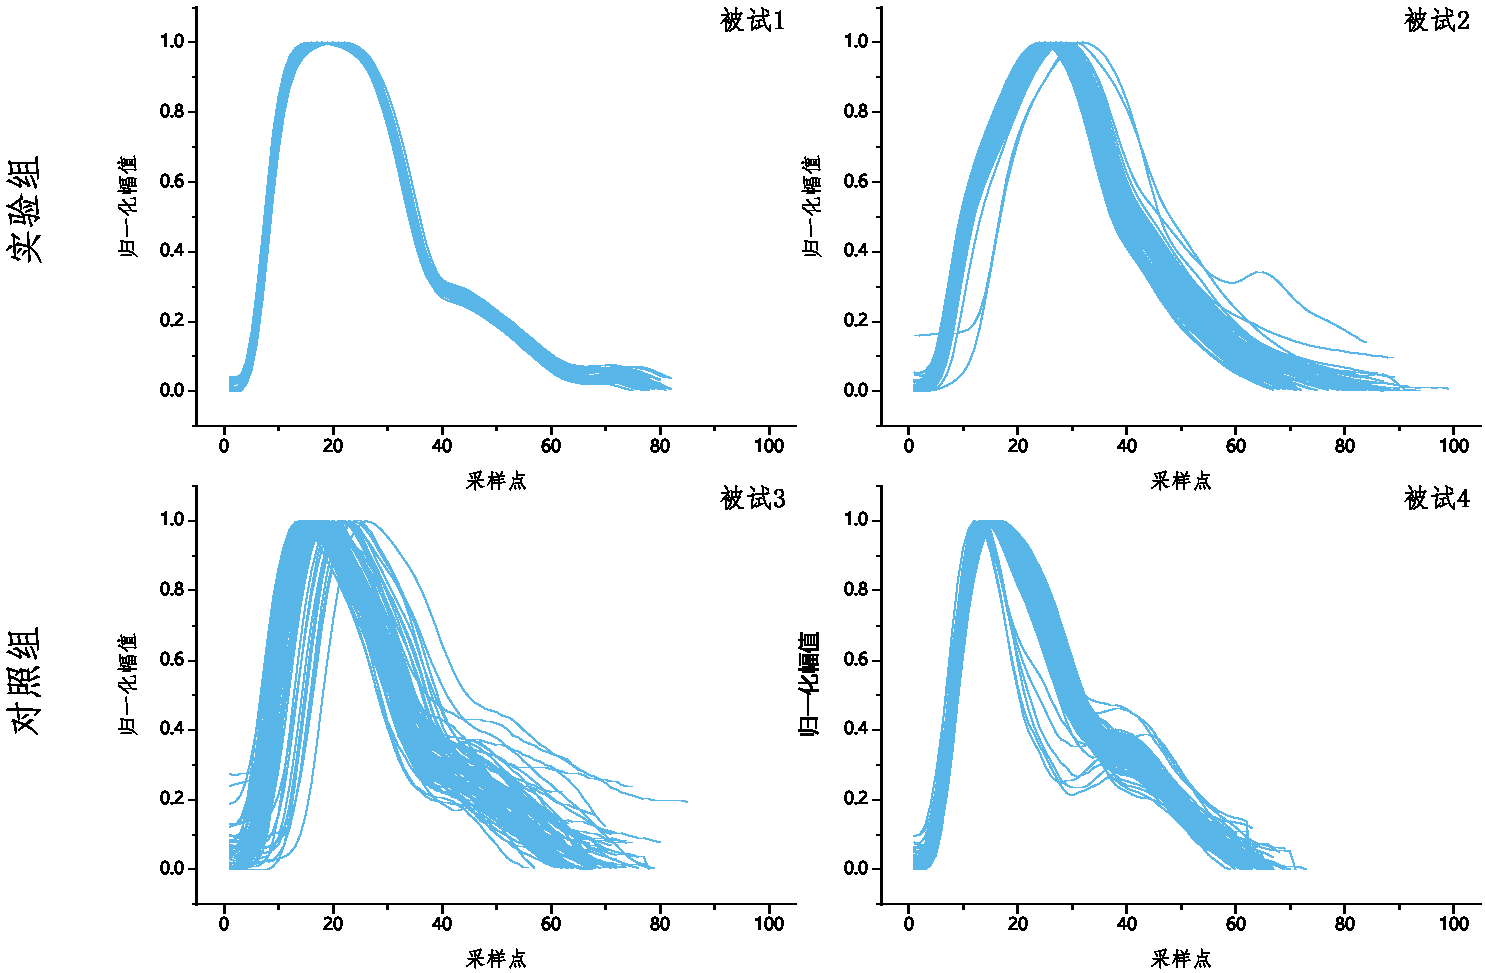
\includegraphics[width=0.75\linewidth]{features/ppgs}
  \caption{\label{fig:no_pe}被试孕妇PPG经标准化处理后的波形对照}
\end{figure}

从\autoref{fig:no_pe}可以看到,实验组与对照组的被试在PPG波形形态及整体分布上均呈现出一定的差异,这说明通过采样值描述PPG波形的可行性。
此外,从\autoref{fig:no_pe}也可以看到,即使对同一被试而言,不同PPG波形之间也存在这较为明显的时长差异。若不加任何处理,这种差异会直接导致PPGSSTFS的维数差异。

为消除\autoref{fig:no_pe}中维数差异可能带来的影响,本研究使用了4.2.3小节介绍的重采样策略(RS)与补齐策略(CS)。
由于本文得到的实验数据采样率为100Hz,采集得到的绝大多数PPG波形采样点数不足80,并且没有任何有效波的的采样点数超过120。
因此,本研究将RS策略下的统一采样点$n_r$设置为100,CS策略下的统一采样点$n_c$设置为120。
前者保证了PPG波形的描述的分辨率与精度,同时可保证只有极少数波形需要进行采样点的压缩;后者则确保了所有波形的采样点数一定相同。

\section{脉搏波时域特征集的处理}
数据是为具体的ML研究问题而准备的,故在对数据进行下一步处理前,有必要明确本文需要研究的具体ML的问题与任务。本小节对介绍了使用PPG研究PE问题的两个角度。在此基础上,
对PPGMTFS与PPGSTFS等两个数据集的预处理工作从数据集的划分、特征缩放及特征降维等方面进行了说明。

\subsection{关于子痫前期的假设与构建机器学习模型的角度}
绪论中已经阐述过,本文的研究目标是探寻通过PPG识别判断PE病发的可能,而该目标本质上可以划分为ML领域内的二分类任务。
由于PPG是一种平稳随机信号,短时间内采样得到的数据波形理应具有较高的相似度\cite{Qiu2012,PPGYY,Ma2015}。
故本文对PPG与PE之间的可能潜在的关系,提出了以下两种分析角度。

一、\textbf{单个PPG波形可以反映PE的病发状态}

在这种分析角度下,PPG的波形是孕妇PE病发状态的稳定“表达”,单个PPG波形包含了可以识别区分PE的全部信息。在这种分析角度下,由PE导致的病生理变化可以在单个波形上得到全部体现,
单个PPG波形能够作为分析识别PE的最小分析对象。

二、\textbf{被试的全部PPG波形才可以反映PE病发状态}

在这种分析角度下,PPG的单个波形是孕妇PE病发状态的不稳定“表达”,但孕妇的一段时间内采集得到的所有PPG波形包含了可以识别区分PE的全部信息。在这种分析角度下,由PE导致的病生理变化可以在孕妇
的多数PPG波形的形态特征上得到全部体现,需要被试的全部PPG波形进行一个类似“群体决策”的过程。

针对以上两个研究角度,本研究拟从以下两个方向展开具体研究工作:

一、基于波形的研究

基于波形的研究(pulse-based research,PR)将单个PPG波形作为分析识别PE的最小分析对象,并进行ML算法模型的研究。此研究方向下,同一被试的PPG数据可能对应ML模型训练与验证阶段的多个数据样本,这种方式相对地增加了
数据集的样本容量。

二、基于被试的研究

基于被试的研究(subject-based research,SR)将单个被试的所有PPG波形作为一个整体进行分析处理,并进行ML算法模型的研究。此研究方向下,同一被试的PPG波形只会出现在训练集或测试集之中,
测试集中的数据样本对于训练得到的模型是完全陌生的未见示例,因此更考验ML模型的泛化能力。

\subsection{数据集的划分}
数据集的划分是监督学习在开始模型训练前必不可少的重要步骤,是将原始数据集划分为训练集与测试集的过程。其中,训练集作为训练模型的输入数据,而测试集则是用来评估该模型在未见示例上的泛化能力。

第三章已经介绍过,本文共采集得到79例被试孕妇的有效PPG数据波形共计7864个,其中,实验组44名被试包含有效波形4683个,对照组35名被试包含波形3181个。
由于本文使用了PPGMTFS与PPGSTFS等两个数据集,并提出了PR与SR等两个具体研究方向,且后续章节在进行研究时也使用了多种ML算法进行模型的构建,数据集的合理划分显得尤为重要。
本文从以下方面进行了处理工作。

一、按合理比例划分

前人的研究已经证实,在进行数据划分时,测试集包含的样本数量与全部样本的比例的最优区间在[20\%, 30\%]\cite{Gholamy2018Why7O}。
本论文选取了划分比例最为常见的20\%,按照训练集与测试集4:1的比例分别按被试与波形对原始数据抽样。

二、分层抽样

由于本文实验得到的PPG数据在是否患有PE的这一问题上存在分布不平衡现象,直接使用纯随机方法抽样有可能导致抽样偏差,最终影响准确性、稳定性与鲁棒性等模型效果\cite{Aurélien2018}。
为了避免此情况发生,本研究额外应用了分层抽样的策略划分数据集,将数据样本按其是否属于实验组分成两组,对新得到的两组数据
分别按照4:1比例进行抽样,两组对应的抽样结果在合并之后才形成最终的训练集与测试集。

三、固化抽样结果

为使后续多种ML模型的性能具有可比行,必须保持数据集的划分在整个研究过程中的一致性。因此,前两步中的分层抽样过程只进行一次,随即被固化保存。该划分结果在之后的ML过程中不再进行任何其他调整,
供所有ML算法训练模型或进行测试使用。

最终的数据集划分结果如\autoref{tab:dataset}所示。
\begin{center}
  \zihao{-5}
  \begin{longtable}{m{1.5cm}<{\centering}m{1.5cm}<{\centering}m{1.5cm}<{\centering}m{1.5cm}<{\centering}m{1.5cm}<{\centering}m{1.5cm}<{\centering}}
    \caption{数据集划分结果}\\
    \label{tab:dataset}\\
        \topline
        \colorhead & & \multicolumn{2}{c}{\textbf{训练集}} & \multicolumn{2}{c}{\textbf{训练集}}\\
        \colorhead \multirow{-2}{*}{\textbf{研究方向}}& \multirow{-2}{*}{\textbf{研究方向}}& \textbf{实验组} & \textbf{对照组} & \textbf{实验组} & \textbf{对照组} \\
        \midline
        \endfirsthead
        \caption[]{(续)}\\
        \midline
        \colorhead & & \multicolumn{2}{c}{\textbf{训练集}} & \multicolumn{2}{c}{\textbf{训练集}}\\
        \colorhead \multirow{-2}{*}{\textbf{研究方向}}& \multirow{-2}{*}{\textbf{研究方向}}& \textbf{实验组} & \textbf{对照组} & \textbf{实验组} & \textbf{对照组} \\
        \midline
        \endhead 
        \midline
        \endfoot
        \bottomline
        \endlastfoot
        \colorrowa  PR  & 7864  & 3746 & 2545 & 937 & 636 \\
        \colorrowc  SR  & 79  & 35 & 28 & 9 & 7 \\           
  \end{longtable}
\end{center}
\vspace{-0.8cm} 

\subsection{特征缩放}
一般而言,原始数据的输入特征在数值属性出现较大的差异会导致机器学习模型的性能下降、表现欠佳\cite{Aurélien2018}。为保证这些输入特征能满足特定的机器学习算法的输入要求,通常还要对这些特征的数值分布进行一定的调整,这也就是特征缩放操作。

常见的特征缩放处理原则是同比例缩放所有属性,使用的方法有归一化与标准化等两类方法。归一化方法又称为最小-最大缩放,可将所有数据的特征属性值同比例映射至[0,1]区间内
\begin{equation}
  \label{equ:maxmin}
  z = \frac{x - x_{min}}{x_{max}-x_{min}}
\end{equation}
其中,$z$为缩放后的数据,$x$需要标准化的数据,$x_{min}$与$x_{max}$分别对应这批数据的最小值与最大值。

而标准化的过程可将所有数据的特征属性调整至符合正态分布
\begin{equation}
  \label{equ:normalization}
  z = \frac{x - \mu}{\epsilon}
\end{equation}
其中,$z$为缩放后的数据,$x$需要标准化的数据,$\mu$与$\epsilon$分别对应这批数据的平均值与样本方差。

\subsection{特征降维}
机器学习模型的训练过程花费的时间成本会随着输入特征维数的增加而成非线性增加,这也就是通常而言的维数诅咒或维数灾难。
为加快模型训练速度,一种可行的策略在构建模型时尽可能只使用“与预期结果最相关的”、“最重要的”输入特征,即按照特征的贡献度对
原始数据集进行降维处理。需要注意的是,数据降维在加速训练的同时,通常也会导致模型性能的下降。因此,一般认为特征降维是机器学习过程中的一个可选项而非必选项。

特征降维在训练模型前后均可进行。在训练模型前的特征降维处理
主要依赖于特征数据属性值的分布特性进行筛选;在模型训练完成后的特征降维主要依赖于特征属性对模型的贡献程度进行筛选。
本小节在训练机ML模型前,使用统计分析中的U检验方法,评估了PPGMTFS中各特征参数与PE的相关性,进而完成了特征筛选与降维,如\autoref{tab:utest}所示。

\begin{center}
  \zihao{-5}
  \begin{longtable}{m{2.5cm}<{\centering}m{2cm}<{\centering}m{2.5cm}<{\centering}m{2cm}<{\centering}m{2.5cm}<{\centering}m{2cm}<{\centering}}
    \caption{脉搏波时域特征集\Rnum{1}数据特征的U检验结果}\\
    \label{tab:utest}\\
        \topline
        \colorhead \textbf{特征缩写}&\textbf{p值}&\textbf{特征缩写}&\textbf{p值}&\textbf{特征缩写}&\textbf{p值}\\
        \midline
        \endfirsthead
        \caption[]{(续)}\\
        \midline
        \colorhead \textbf{特征缩写}&\textbf{p值}&\textbf{特征缩写}&\textbf{p值}&\textbf{特征缩写}&\textbf{p值}\\
        \midline
        \endhead 
        \midline
        \endfoot
        \bottomline
        \endlastfoot
        \colorrowa  LVLR\_9  &  0.004 &  CVLF\_1  & \cellcolor{pink} \textbf{0.068} &  SVRR\_2  &  0.027 \\
        \colorrowc  LVLF\_1  &  \cellcolor{pink}\textbf{0.27}  &  CVLF\_2  &  0.038 &  SVRR\_3  &  0.001 \\
        \colorrowa  LVRR\_6  &  0.002 &  CVRF\_4  & \cellcolor{pink} \textbf{0.44}  &  SVRR\_4  &  0.001 \\
        \colorrowc  LVRR\_7  &  \cellcolor{pink}\textbf{0.387} &  CVD\_1   &  \cellcolor{pink}\textbf{0.159} &  SVD\_2   &  0.009 \\
        \colorrowa  LVD\_1   &  0.022 &  CVD\_2   &  0.024 &  SVD\_3   & \cellcolor{pink} \textbf{0.65}  \\
        \colorrowc  LVD\_2   &  0.006 &  CVALF\_6 &  0.02  &  SVALR\_2 & \cellcolor{pink} \textbf{0.078} \\
        \colorrowa  LVALR\_4 &  0.013 &           &        &  SVALR\_3 &  0.001 \\
        \colorrowc  LVALR\_5 &  \cellcolor{pink}\textbf{0.063} &           &        &           &               
  \end{longtable}
\end{center}
\vspace{-0.8cm} 

\autoref{tab:utest}列举出了由U检验得到的所有$p$值$>10^{-4}$的特征参数,其中,特征缩写所对应的具体特征与\autoref{tab:allfeatures}保持一致,特征缩写后的数值表示
该特征在PPGFV中的向量下标,该数值越小表示该特征在对应的PPGFV中越接近PPG波峰。由三种策略确定的PPG多维度时域特征均存在着一定数量的在PE数值上无统计差别的特征($p$值$> 0.05$),
\autoref{tab:utest}对这8种用粉红底色加粗字体进行了突出显示,这部分特征未参与后续模型的训练。
故在初筛完成后,PPGMTFS共有特征286个。

在模型训练后的特征筛选处理可参见下一章节相关内容。

\section{小结}
本小节完成了PPGMTFS与PPGSTFS等两个数据集的构建工作,对两个特征集的在构建过程中的设计思路与处理细节也进行了详细说明。
明确了利用PPG数据通过ML方法对PE识别的两个研究角度,并确定了按照PPG波形与被试开展研究的两个方向。此外,按ML模型构建的要求,对上述两个特征集进行了预处理工作。
本章的研究内容为后续的机器学习分析工作做好了数据准备与铺垫工作。